\chapter{Informationsbeschaffung}
\label{chap:Informationsbeschaffung}
Dieses Kapitel bietet fundamentale, physikalische Gegebenheiten sowie die relevanten Eigenheiten des verwendeten \ac{PIR} Sensors. Da es sich um ein bildgebendes Messprinzip handelt, werden des Weiteren geometrische Aspekte erläutert. Schlussendlich liefert dieses Kapitel auch nötige Informationen über das Messobjekt bzw. die Messumgebung.

\section{Grid-Eye AMG8834}
\label{sec:AMG8834}

Der verwendete Panasonic AMG8834 ist ein bildgebendes \ac{MEMS}-Sensor, der mit insgesamt 64 temperaturempfindlichen Thermosäulenelementen ausgestattet ist. Diese sind als 8x8 Pixelmatrix auf den Chip aufgebracht. In Abbildung \ref{fig:Explosionsdarstellung} ist der Aufbau des Sensors dargestellt. Nachfolgende Angaben sind aus dem Datenblatt zu entnehmen, sofern nicht anders angegeben.
 
\begin{figure}[H]
	\centering
	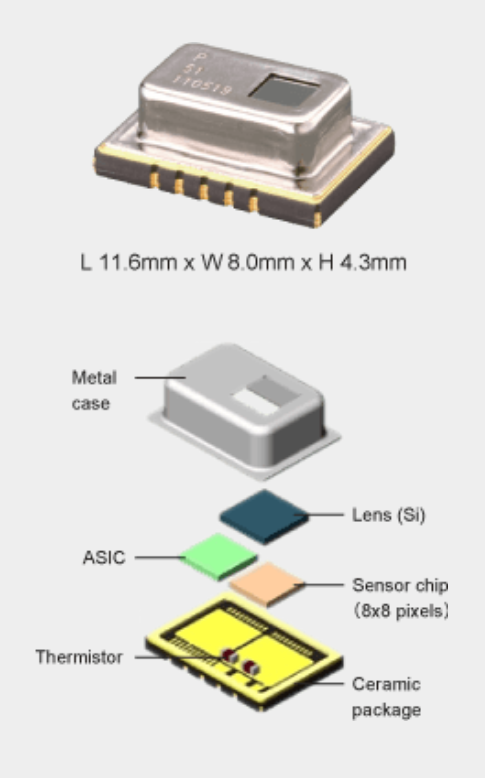
\includegraphics[width=0.3\textwidth]
	{fig/grid_eye_aufbau.PNG}
	\caption[Aufbau des AMG8834 Sensors]{Aufbau des AMG8834 Sensors} [\protect\cite{AMG8834}]
	\label{fig:Explosionsdarstellung}
\end{figure}
Die eintreffenden Infrarotwellen werden durch die Siliziumlinse, welche einen \ac{FOV} von 60$^\circ$ besitzt, gefiltert. Dabei durchdringen lediglich langwellige Infrarotstrahlungen mit den Wellenlängen 8 - 14 $\mu$m die Linse. 

In Abbildung \ref{fig:SchemaAMG8834} ist das Prinzipschema des Sensors dargestellt. Die Umwandlung der Infrarotwellen in die Thermospannung wird im Unterkapitel \ref{subsec:seebeck} detailliert erläutert, daher wird in diesem Abschnitt darauf verzichtet. Die Signale der einzelnen Pixel werden durch die \ac{ASIC} des \ac{MEMS}-Sensor verarbeitet. Die selektierte Thermospannung wird verstärkt, mit dem integrierten Thermistor verglichen und mit dem \ac{ADC} gewandelt. Durch die hohe interne Verstärkung besitzt der Sensor bei normalen Bedingungen\footnote[1]{Umgebungstemperatur 0 - 80 $^\circ$C bei Luftfeuchtigkeit 15 - 85\%} eine Genauigkeit von +/- 2.5 °C. 

\begin{figure}[H]
	\centering
	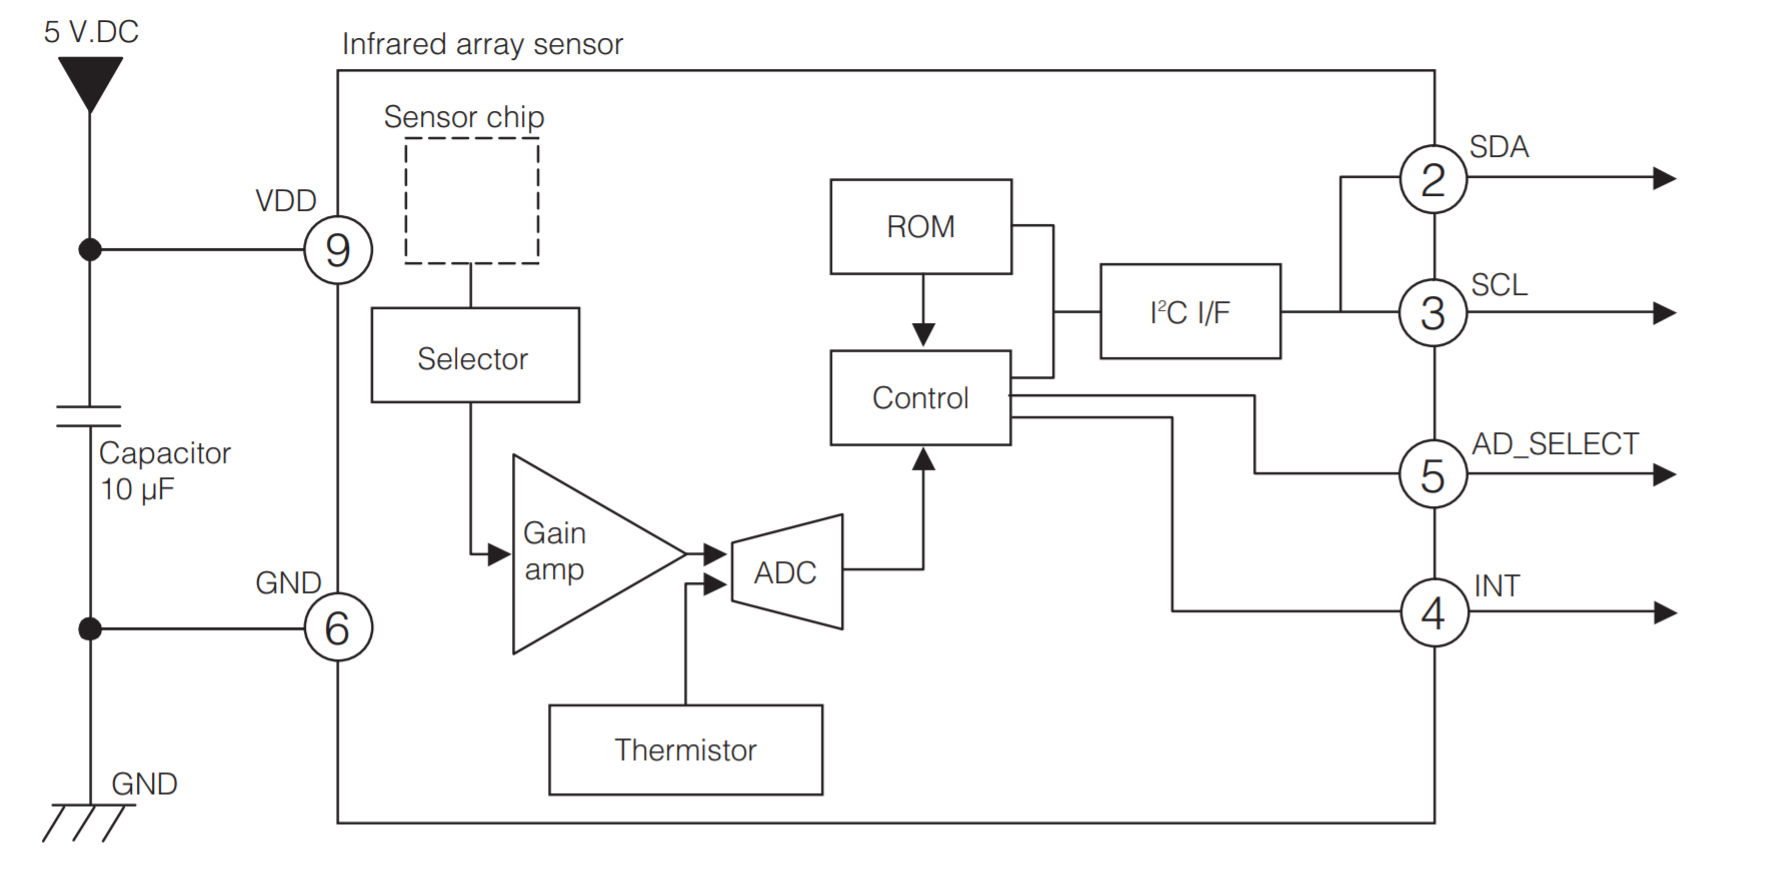
\includegraphics[width=0.75\textwidth]
	{fig/Circuit_AMG8834.PNG}
	\caption[Schema des AMG8834 Sensors]{Schema des AMG8834 Sensors} [\protect\cite{AMG8834}]
	\label{fig:SchemaAMG8834}
\end{figure}
 
Über die \ac{I2C}-Schnittstelle lassen sich die Werte der Thermoelemente und der Thermistoren je aus zwei Registern auslesen. Die Messwerte werden alle 100 ms aktualisiert. Dabei werden lediglich 12 Bit pro Pixel für die Temperaturregister genutzt. Dies führt zu der kleinsten unterscheidbaren Grösse von 0.25 $^\circ$C. Die Thermistorregister lassen sich mit der Auflösung von 0.0625 $^\circ$C unterscheiden. Im Datenblatt wird zwar eine \ac{NETD} von 0.05 °C für die Pixelwerte angegeben. Durch den \ac{ADC} kann diese Angabe jedoch nicht als Qualitätsangabe benutzt werden.
In Abbildung \ref{fig:SchemaAMG8834} ist klar ersichtlich, dass die Umgebungstemperatur, bzw. die Temperatur, welche vom Thermistor gemessen wird, direkten Einfluss auf die Pixelwerte hat. Variieren die Thermistorwerte aufgrund von Raumtemperaturschwankungen, entstehen bei den Pixelwerten dadurch entsprechende Schwankungen.

\section{Physikalische Aspekte}
\label{sec:Physik}
Dieser Abschnitt erläutert auf prägnante Weise, physikalische Aspekte die dem Sensor zu Grunde liegen. Dies bietet die Grundlage für die Bestimmung der Störquellen und das Verhalten des Sensors bei äusseren Einwirkungen. Die Tabelle \ref{tab:Legende Physikalische Grössen} gibt die Bezeichnungen der folgenden Formeln\footnote[2]{Anmerkung zu $M_{\lambda }$: der Steradiant sr ist die Messeinheit für den Raumwinkel} wieder.

\begin{table}[H]
	\centering
	\begin{tabular}{l|c|c}
		\rowcolor{gray} Grösse &  Bezeichnung  & Einheit \\
		\hline 
		Thermospannung &  $ U_{t}$ & $V$  \\ 
		\rowcolor{gray} Thermokraft P/N -Silizium  & $\alpha_{p},\alpha_{n}$ & $V/K$\\	
		Temperatur P/N -Silizium &  $T_{p},T_{n}$ & $K$ \\
		\rowcolor{gray}Wärmestrom &  $\dot{Q}$ & $J/s$  \\ 
		Emission & $\epsilon$ & $-$\\	
		\rowcolor{gray}Reflektion &  $\rho $ & $-$ \\
		Transmission & $\tau$ & $-$\\
		\rowcolor{gray}Absorption &  $\alpha$ & $-$  \\ 
		Strahlungsleistung & $\dot{Q}$ & $W$\\
		\rowcolor{gray}spektrale spezifische Ausstrahlung &  $M_{\lambda }$ & $W/sr$  \\
		Planksches Wirkungsquantum &  $ h$ & Js \\ 
		\rowcolor{gray} Lichtgeschwindigkeit im Vakuum & $c $ & $ m/s$ \\ 
 		Stefan-Boltzmann-Konstante & $\sigma$ & $ W/m^2K^2 $ \\ 
	\end{tabular}
	\caption{Physikalische Grössen }
	\label{tab:Legende Physikalische Grössen} 
\end{table}

\subsection{Seebeck-Effekt}
\label{subsec:seebeck}
In Abbildung \ref{fig:AufbauThermo} ist ein einzelnes Pixel funktionell dargestellt. Die durch die konvexe Linse gesammelten Infrarotstrahlen verursachen auf den dünnen Thermosäulenflächen (2), dass die Oberfläche erwärmt wird. Zwischen der erwärmten, n-dotierten Siliziumschicht (4) und der kühleren, p-dotierten Siliziumschicht (6) entsteht ein Temperaturgefälle.   

\begin{figure}[H]
	\centering
	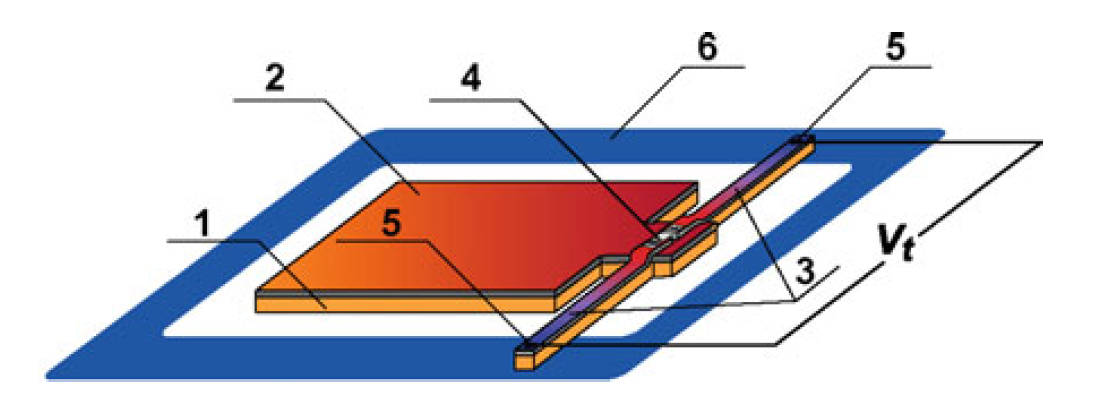
\includegraphics[width=0.5\textwidth]
	{fig/Mems_Thermopile.PNG}
	\caption[Aufbau Thermosäulenelement]{Aufbau des Thermosäulenelement} [\protect\cite{AMG8834}]
	\label{fig:AufbauThermo}
\end{figure}

Durch die unterschiedlichen Thermokräfte\footnote[3]{Auch Seebeckkoeffizienten genannt} der zwei Halbleitermaterialien entsteht ein Potentialunterschied, den man an den zwei äusseren Eckpunkten (5) abgreifen kann. Diese Spannung $U_{t}$ ($V_{t}$) ist die Grundlage des Messprinzips und wird mit Formel \ref{eq1} beschrieben [\protect\cite{AMG8834}].

\begin{equation}
\label{eq1}
U_{t} = (\alpha_{p} + \alpha_{n})*(T_{p}+T_{n})
\end{equation}
\myequations{\tab Seebeck-Effekt}

\subsection{Strahlungsquellen}
\label{subsec:Strahlungstheorie}
Der vorherige Abschnitt erläutert die Funktion des Sensors als Infrarotempfänger. Nicht unwesentlich ist weiter die Betrachtung der Strahlungsquellen. Grundsätzlich gilt: Jeder Körper, der eine Temperatur oberhalb des absoluten Nullpunkt\footnote[4]{Als 0 Kelvin [K] festgelegt, das entspricht -273,15 °C.} aufweist, strahlt Wärmestrahlung im Infrarotbereich ab. Im Allgemein wird für die Betrachtung vom Plank'schen Strahlungsgesetz ausgegangen. Nach dieser gilt für eine spektrale, spezifische Ausstrahlung eines Schwarzkörpers mit der Temperatur T folgende Formel [\protect\cite{Thermoformeln}]: 

\begin{equation}
\label{eq2}
M_{\lambda } = \frac{2\pi h c^2 }{\lambda^5}*\frac{1}{e^\frac{hc}{\lambda k_{B} T}-1}
\end{equation}
\myequations{\tab Plank'sches Strahlungsgesetz}

Wie in der Formel ersichtlich ist die Ausstrahlung eines schwarzen Körper mit 5. Potenz von der Wellenlänge $\lambda$ und exponentiell von der Temperatur $T$ abhängig. Durch die Siliziumlinse des Sensors werden Störquellen, welche andere Wellenlängen aufweisen, gefiltert. Dies ist vor allem bei Lichtquellen eine relevante Eigenschaft. Da dessen Spektrum sich tiefer\footnote[5]{Bereich 0.4$ \mu$m - 2 $\mu$m} befindet, können Strahlungseinflüsse von herkömmlichen Lichtquellen ignoriert werden.

Das Stefan-Boltzmann-Gesetz [\protect\cite{Thermoformeln}] gibt die Strahlungsintensität $\dot{Q}$ eines Temperaturstrahlers an. Diese Formel bietet für die Anwendung relevante Erkenntnisse.

\begin{equation}
\label{eq3}
\dot{Q} = \frac{\mathrm{d} Q}{\mathrm{d} t} = \epsilon *\sigma * A * T_{obj}^4
\end{equation}
\myequations{\tab Wärmestrahlung}

Diese Formel zeigt auf, dass die Wärmestrahlung eines Körpers im Wesentlichen (mit 4. Potenz) von der eigenen Temperatur abhängig ist. 
Die Fläche A ist lediglich proportional. Dies verursacht, dass bereits flächenmäßig kleine, jedoch stark erwärmte Objekte im Messbereich einen bedeutenden Einfluss auf die Messresultate liefern. Zusätzlich verursachen Wärmequellen im nahen Umfeld des Sensors Abweichungen auf die Sensorwerte. In Abbildung \ref{fig:thermosäule} ist das Sender-Empfänger-Prinzip dargestellt.

\begin{figure}[H]
	\centering
	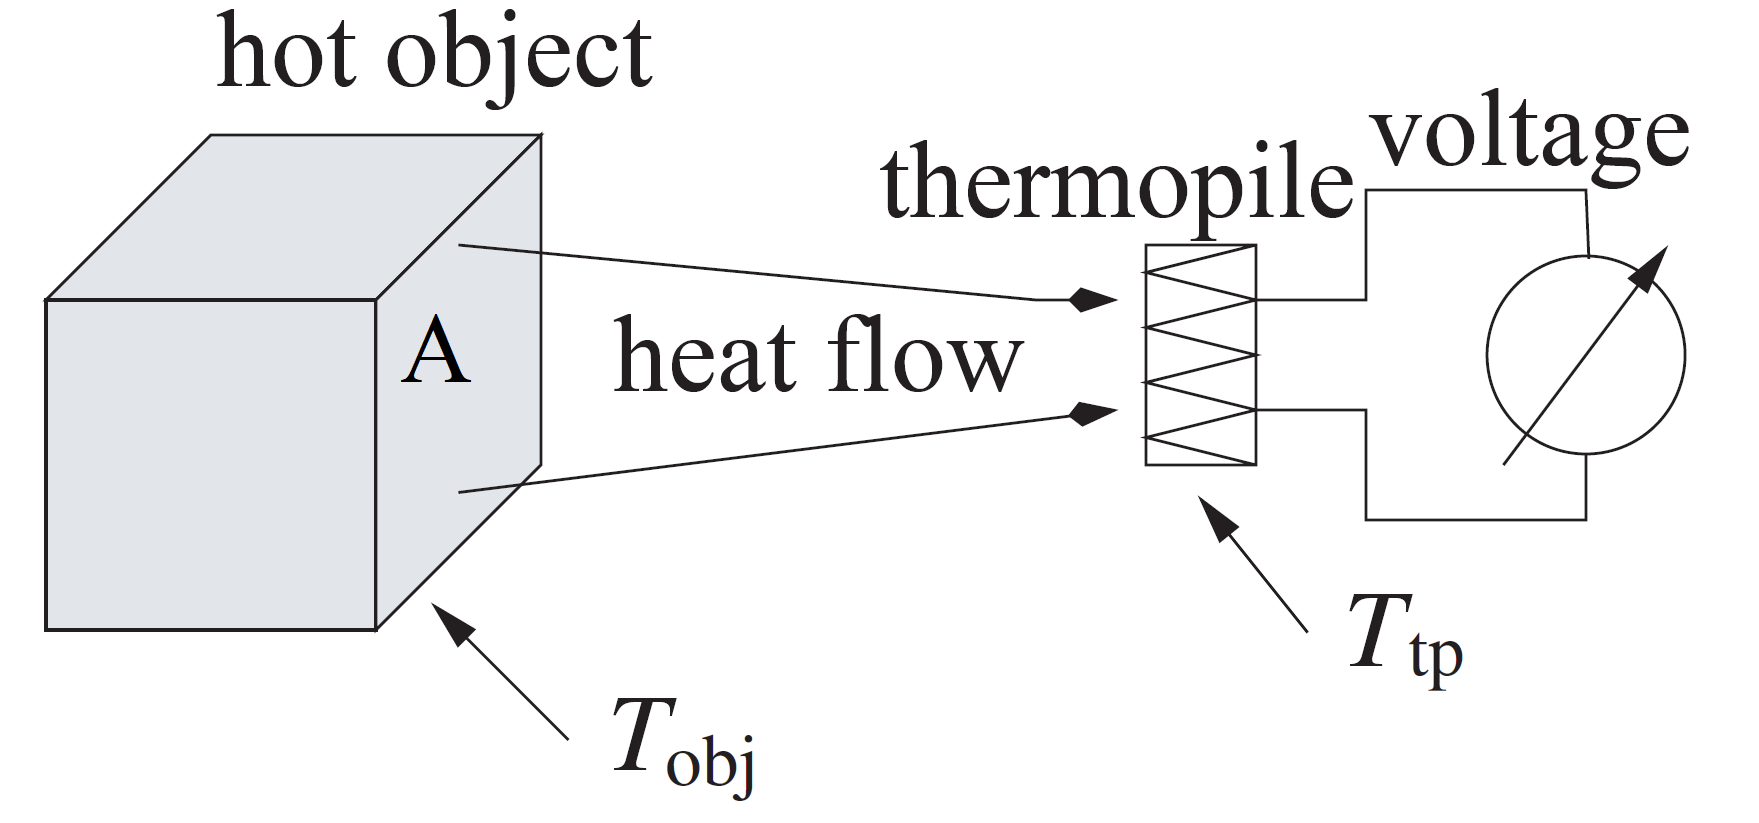
\includegraphics[width=0.4\textwidth]
	{fig/seebeck2.PNG}
	\caption[Sender-Empfänger-Prinzip]{Sender-Empfänger-Prinzip} [\protect\cite{seebeck}]
	\label{fig:thermosäule}
\end{figure}


Das Stefan-Boltzmann-Gesetz deutet auf eine weitere relevante, physikalische Gegebenheit hin, die mit dem Emissionsgrad $\epsilon$  in Verbindung steht.
 Der Emissionsgrad $\epsilon$ ist ein materialabhängiger Faktor, welcher zwischen 0 bis 1  angegeben wird. Dieser gilt für graue Körper d.h. für Körper, dessen Oberfläche auftreffende Strahlungen nicht vollständig absorbieren. Diese Eigenheit gilt für alle realen Körper. Da der Emissionsgrad vom Material und dessen Oberfläche abhängt, können starke Unterschiede entstehen. Im Unterkapitel \ref{subsec:Personenaufzuege} werden übliche Aufzugsmaterialien betrachtet.

Neben der Emission können auch Reflexion und Transmission von Störquellen Einfluss auf die Messwerte besitzen. In den nachfolgenden Formeln wird dies aufgezeigt. Nach dem Energieerhaltungsgesetz [\protect\cite{Thermoformeln}] gilt für Transmission, Reflexion und Absorption die Formel \ref{eq4}.
\begin{equation}
\label{eq4}
\tau  + \alpha + \varphi  = 1
\end{equation}
\myequations{\tab Energieerhaltung der Wärmestrahlung}

Bei thermischen Gleichgewicht kann angenommen werden, dass der Emissionsgrad der Absorption entspricht.

\begin{equation}
\label{eq5}
\epsilon \approx  \alpha
\end{equation}
\myequations{\tab Emissionsgrad bei thermischem Gleichgewicht}

Da in Aufzügen nur von Festkörpern ausgegangen wird, fällt die Transmission $\tau$ aus der Gleichung. Es können somit lediglich Reflexionen oder die Emission eines Festkörpers Einfluss auf die Messresultate des Sensors haben. Weitere Betrachtungen folgen in Unterkapitel \ref{subsec:Personenaufzuege}.

\section{Geometrische Aspekte}
\label{sec:geometrie}

In Aufzügen lässt sich der Sensor lediglich an der Decke befestigen, damit die gesamte Aufzugsfläche ausgemessen werden kann. Bei seitlicher Montage können Abschattungen durch Personen verursacht werden, daher wird für die geometrische Betrachtung vom Deckenzentrum eines Aufzugs ausgegangen. In der nachstehenden Skizze sind die Verhältnisse perspektivisch dargestellt. Dabei wird von einer Raumhöhe\footnote[6]{Nach Standardkabine EN 81-70} von 2.10 m ausgegangen.
 
 
\begin{figure}[H]
	\centering
	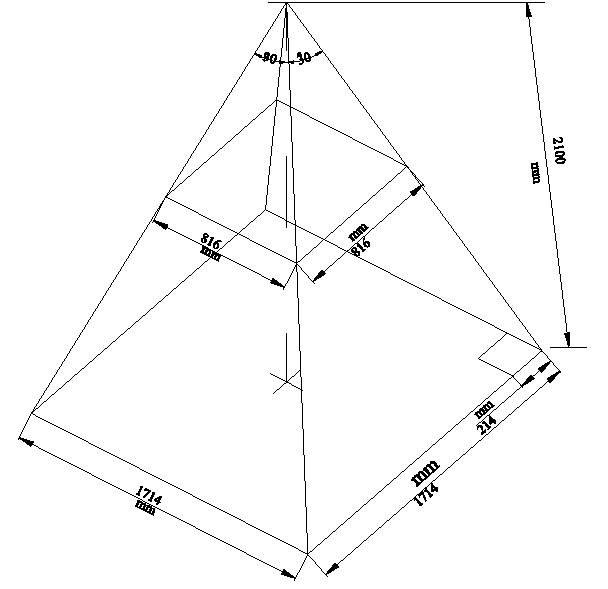
\includegraphics[width=1.0\textwidth]{fig/Skizze_bearb.jpg}
	\caption[Skizze Geometrie des Sensors]{Skizze: Geometrie des Sensors}
	\label{fig:skizze}
\end{figure}

Da die Strahlungsintensität mit zunehmender Distanz im Quadrat\footnote[7]{Nach Abstandsgesetz} abnimmt, spielt die Distanz zum Messobjekt eine entscheidende Rolle. Für den Einsatz in Personenaufzügen ist neben der Distanz zum Objekt auch der \ac{FOV} des Sensors ziemlich entscheidend. In der Abbildung \ref{fig:skizze} ist zu sehen, dass bei der festgelegten Raumhöhe eine Fläche von maximal 2.94 $m^2$ abgedeckt wird. Bei der Messung von Personen ist jedoch ein Messabstand zwischen 10 bis 100 cm (\textcolor{red}{rote Markierung}) nötig. In diesem Bereich kann jedoch mit dem aktuellen \ac{FOV} von 60$^\circ$ x 60$^\circ$ im besten Fall eine Fläche von 0.666 $m^2$ erfasst werden.

Für eine Aufzugkabine mit acht Personen\footnote[8]{Masse: (HxBxT) 2100 x 1100 x 1400 [mm]} bei mittlerem Messbereich wird im optimalen Fall ein Öffnungswinkel von 84° x 109$^\circ$ benötigt. Problematisch kann in diesem Zusammenhang die Abschattung des Messbereichs durch grosse Personen sein, welche zentral positioniert sind.

In der Abbildung \ref{fig:skizze} wird davon ausgegangen, dass die Fläche sich verzerrungsfrei vergrössert. Durch die konvexe Linse würde jedoch eine perspektifische Verzerrung entstehen, welche jedoch hier nicht weiter beachtet wird.


\section{Messobjekt und Messumgebung}
\label{sec:Messobjekt}
Dieses Kapitel beschreibt die Erkenntnisse bei der Betrachtung des Messobjekts und der Messumgebung. Dabei wurden einerseits die thermischen Kennwerte von Personen zusammengetragen und anderseits die Messumgebung auf Störquellen und Einflussfaktoren betrachtet. Dank der Firma ARLEWO AG konnten unterschiedliche Aufzüge vermessen und bewertet werden. 

\subsection{Personen}
\label{subsec:Personen}
Die Reaktionen im menschlichen Körper sind auf eine Kerntemperatur von 37 $^\circ$C eingestellt. Am kältesten ist die Haut, die etwa 4 bis 7 Grad  kälter ist. Die Aufteilung der verschiedenen Arten der Wärmeabgabe beträgt bei einem ruhenden Menschen in einer Umgebung von 20 $^\circ$C aus:
\begin{itemize}
	\item 46 \% Strahlung
	\item 33 \% Konvektion\footnote[9]{Konvektion bezeichnet die Wärmeabgabe an
		das umgebende Medium, in der Regel Luft}
	\item 19 \% Schwitzen
	\item \space  2 \% Atmung
\end{itemize}

Die Höhe der Wärmeabgabe hängt im Wesentlichen von der Schwere der Tätigkeit und von der Grösse der Körperfläche ab. Daraus folgt, dass grössere Personen mehr Wärme abgeben. Strahlung und Konvektion nehmen mit zunehmender Umgebungstemperatur bis zum Wert null bei 36 $^\circ$C ab. Hat die Umgebung die Körpertemperatur erreicht, kann folglich durch Strahlung und Konvektion keine Wärme mehr abgeführt werden. In einer Umgebung mit Temperaturen oberhalb 37 $^\circ$C kann also die Wärme nur noch durch Schwitzen abgeführt werden [\protect\cite{MenschWaerme}]. 

Da die Personenerkennung auf Temperaturdifferenzen beruht, kann bei einer Umgebungstemperatur um 37 $^\circ$C eine Person nicht mehr zweifelsfrei von der Umgebung differenziert werden. 

Ein weiterer Aspekt, der die zu messende Temperatur einer Person beeinflusst, ist die Bekleidung. In Abbildung \ref{fig:Waermebild} und Abbildung \ref{fig:Waermebild2} ist zu sehen, dass das thermische Profil einer Person durch die Bekleidung stark variiert.

\begin{figure}[!ht]
	\centering
	\begin{minipage}[b]{0.45\linewidth}
		\centering	
		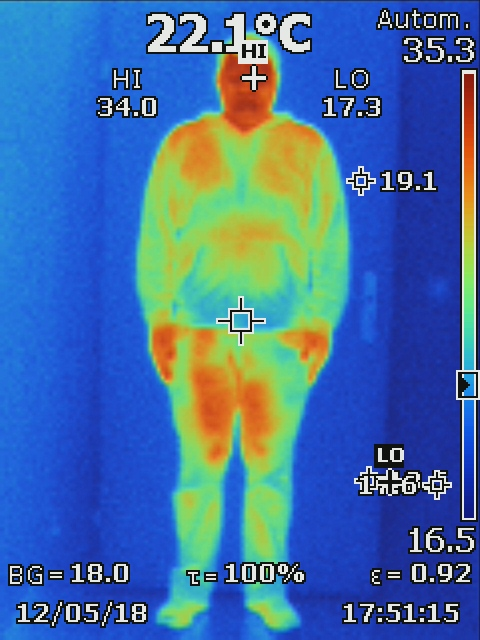
\includegraphics[width=0.8\linewidth]{fig/waermebild1.jpg}
		\captionof{figure}[Wärmebild eines Probanden vollbekleidet]{Wärmebild eines Probanden vollbekleidet}
		\label{fig:Waermebild}
	\end{minipage}
	\hfill
	\begin{minipage}[b]{0.45\linewidth}
		\centering
		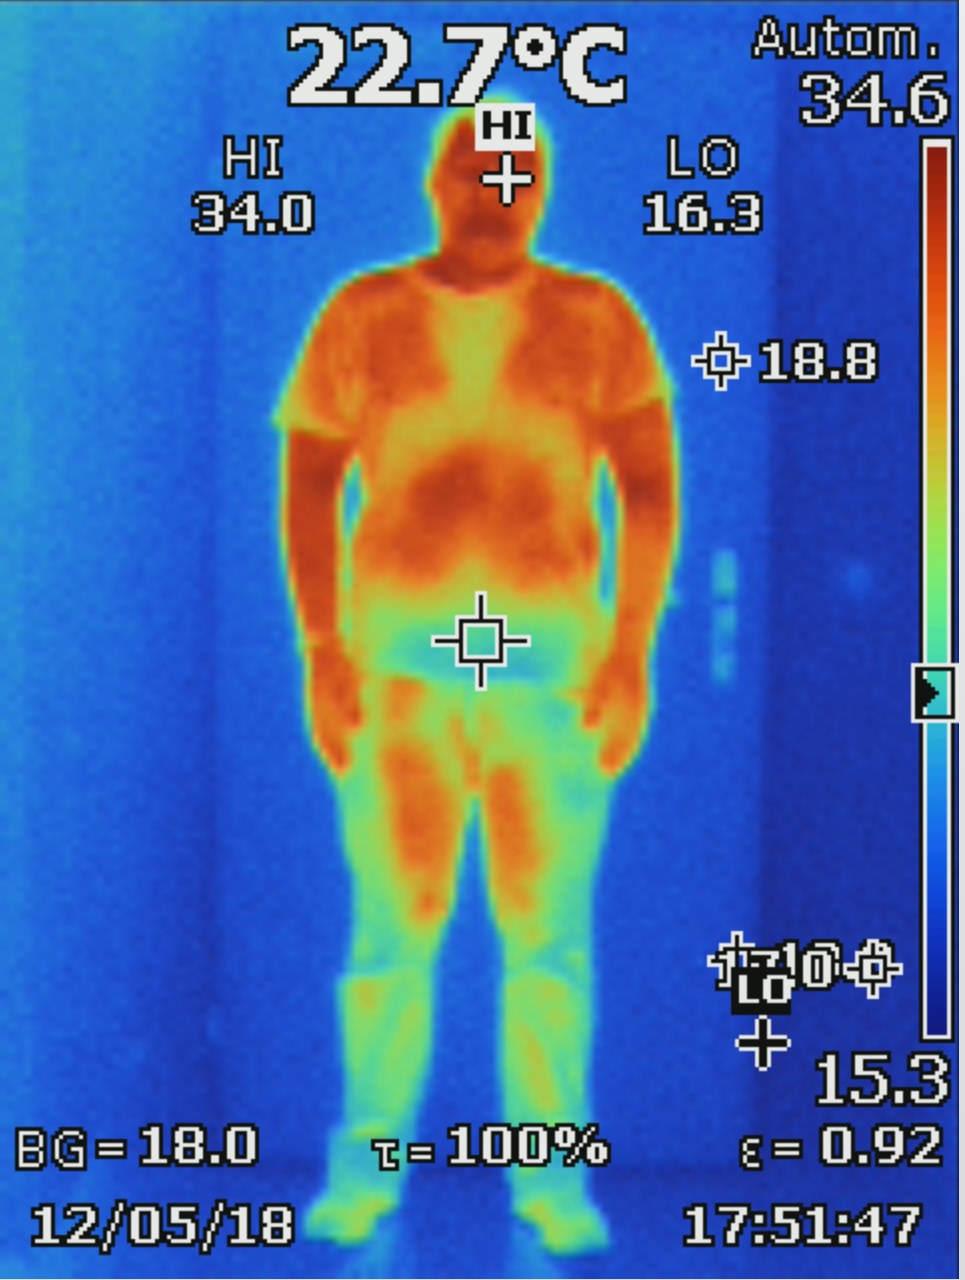
\includegraphics[width=0.8\linewidth]{fig/waermebild2.png}
		\captionof{figure}[Wärmebild eines Probanden teilbekleidet]{Wärmebild eines Probanden teilbekleidet}
		\label{fig:Waermebild2}	
	\end{minipage}
\end{figure}

 Unbekleidete Zonen sind üblicherweise die wärmsten Regionen. Das thermische Verhalten der Bekleidung hängt von der Art der Bekleidung ab und variiert zwischen Hauttemperatur und Umgebungstemperatur. Dabei gibt es grosse Unterschiede im Körperbereich. Für die Personenerkennung ist hauptsächlich der Oberkörperbereich von Interesse, welcher von der Vogelperspektive die grösste Fläche bietet.
 
 Im Falle von einem Umgebungstemperaturwechsel besitzt die Kleidung eine verzögerte Reaktion, bis sich die neue Temperatur einstellt. 
 Dies ist insofern relevant, weil bei einem Wechsel von einem warmen Aussenbereich zu einem beispielsweise klimatisierten Innenbereich, die Bekleidung sich an die neue Temperatur anpasst. In einem Messaufbau konnte diese Problematik verifiziert werden. Es wurden diverse Kleidungsstücke in einem Aufzug getragen, während der Sensor die Personen von der Decke vermessen hat. Da die Personenerkennung in Aufzügen von der Decke ausgeführt wird, sind im Wesentlichen die Kopfbedeckungen ein Störfaktor.

\begin{figure}[!ht]
	\centering
	\begin{minipage}[b]{0.49\linewidth}
		\centering	
		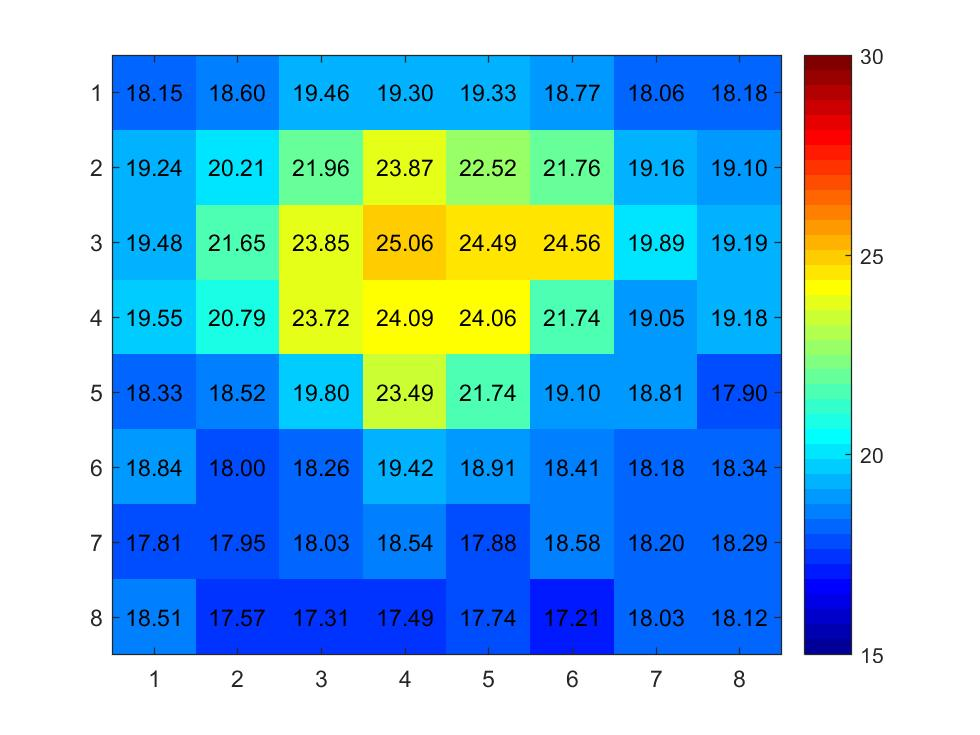
\includegraphics[width=1.0\linewidth]{fig/person_175_shirt.jpg}
		\captionof{figure}[Messresultate ohne Kopfbedeckung]{Messresultate\\ ohne Kopfbedeckung}
		\label{fig:ohneHut}
	\end{minipage}
	\hfill
	\begin{minipage}[b]{0.49\linewidth}
		\centering
		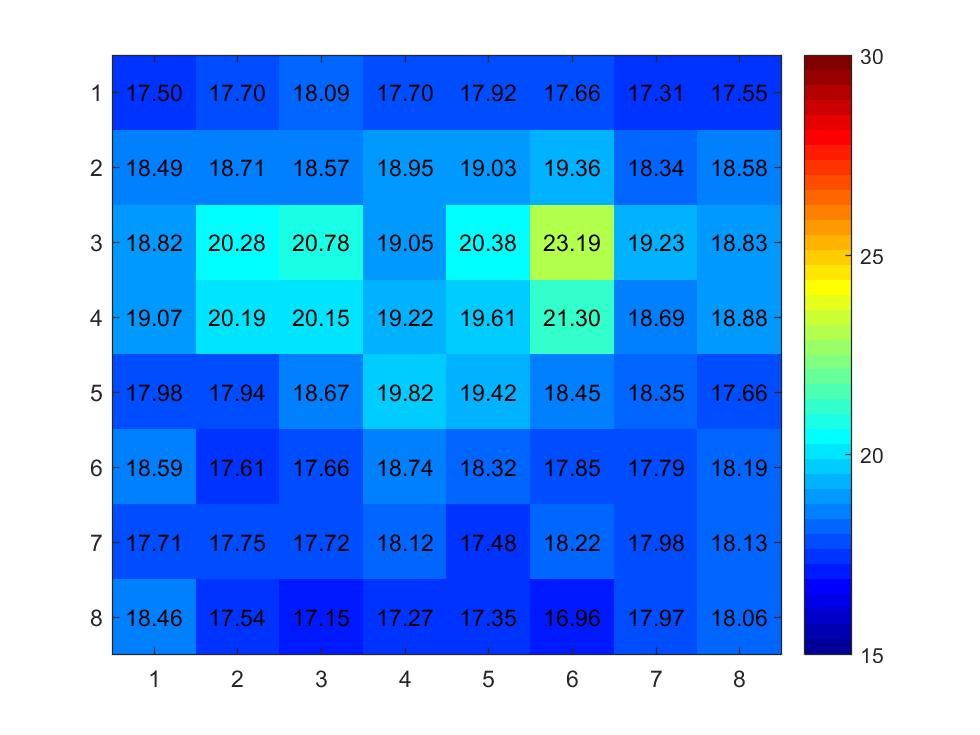
\includegraphics[width=1.0\linewidth]{fig/person_175_kopfbedeckung.jpg}
		\captionof{figure}[Messresultate mit Kopfbedeckung]{Messresultate\\ mit Kopfbedeckung}
		\label{fig:mitHut}	
	\end{minipage}
\end{figure}

In Abbildung \ref{fig:ohneHut} und \ref{fig:mitHut} sind die Sensorwerte der einzelnen Pixel dargestellt. Durch das Tragen einer Mütze, welche der Umgebungstemperatur angepasst ist, wird der Proband vom Sensor nur noch schlecht wahrgenommen.

\subsection{Personenaufzüge}
\label{subsec:Personenaufzuege}
In diesem Unterkapitel wird der Personenaufzug als Messobjekt näher betrachtet. Neben räumlichen Parametern wie Höhe, Grundfläche und Volumen spielen vor allem die Oberflächenbeschaffenheit bzw. das Oberflächenmaterial eine Rolle. Weitere Einflussfaktoren finden sich in der Umgebungstemperatur und den verbauten Leuchtmitteln.

Wie bereits im Unterkapitel \ref{subsec:Strahlungstheorie} erläutert, besitzen die Materialien in einem Personenaufzug zum Teil stark abweichende Emissionsgrade. Dies verursacht einerseits, dass die gemessen Temperaturen nicht den effektiven Temperaturen entsprechen und andererseits, dass Materialien mit tiefen Emissionsgraden anfällig auf Reflektionen von Störquellen sind. Der Sensor AMG8834 ist auf einen Emissionsgrad von 0.93 kalibriert. Dies entspricht in etwa dem Emissionsgrad von Haut\footnote[10]{Zu entnehmen in der Emissionsgradtabelle Anhang \ref{AnhangE}}. In Tabelle \ref{tab:Emission} sind die Emissionsgrade von üblichen Aufzugsmaterialien aufgeführt.
	
\begin{table}[H]
	\centering
	\caption[Emissionsgrade von üblichen Aufzugsmaterialien]{Emissionsgrade von üblichen Aufzugsmaterialien}
	\label{tab:Emission}
	\begin{tabular}{|l|l|l|l|}
		\hline
		\rowcolor[HTML]{C0C0C0} 
		Kunststoffe                & Hartgummi                 & Lackierte Oberflächen           & Aluminium eloxiert        \\ \hline
		\multicolumn{1}{|c|}{0.78} & \multicolumn{1}{c|}{0.85} & \multicolumn{1}{c|}{0.8 - 0.96} & \multicolumn{1}{c|}{0.55} \\ \hline
	\end{tabular}
\end{table}
	

Ein besonderes Augenmerk gilt den Aufzügen mit Edelstahlverkleidung. In Abbildung \ref{fig:Edelstahl} sind unterschiedlich behandelte Edelstahloberflächen dargestellt, welche auch in Aufzügen verwendet werden.  
\begin{figure}[H]
	\centering
	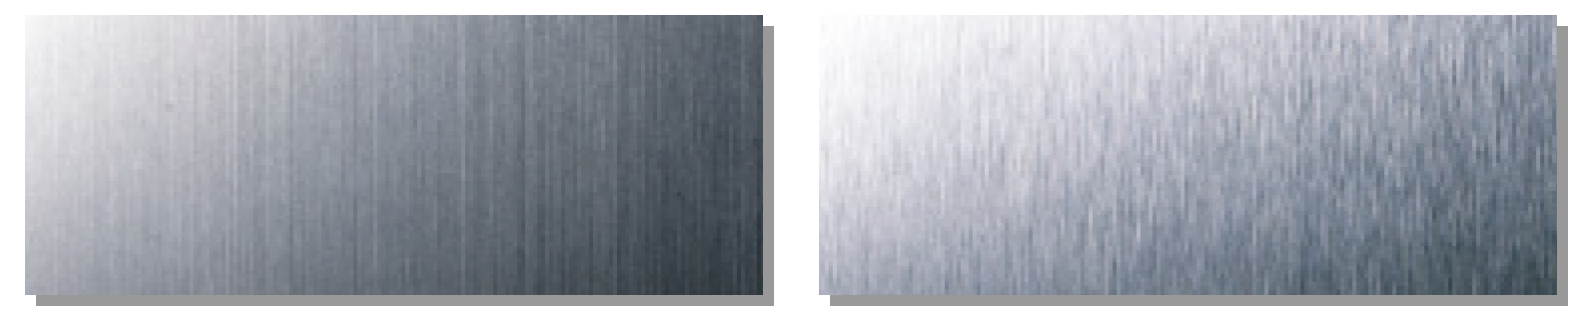
\includegraphics[width=0.8\textwidth]
	{fig/Edelstahl_matt.PNG}
	\caption[Edelstahl warmgewalzt]{Edelstahl warmgewalzt} [\protect\cite{Edelstahl}]
	\label{fig:Edelstahl}
\end{figure}

Die Emissionsgrade von Edelstahl schwanken zwischen 0,05 bis 0.82, je nachdem wie das Material verarbeitet wurde. Auch Veredelungen durch Schleifen, Polieren oder Bürsten verändern die Oberflächenbeschaffenheit und haben eine Änderung des Emissionsgrads zur Folge. Somit lässt sich die Störanfälligkeit von Edelstahlkabinen nur schwer evaluieren. Es muss daher mit äusseren Störeinwirkung gerechnet werden. 

Bei vollverglasten Kabinen kommt noch eine weitere Eigenschaft zum Tragen. Glas besitzt die Eigenschaft auch als Festkörper Infrarotstrahlung zu transmittieren. In Abbildung \ref{fig:Glas} sind die drei Grade im  Wellenlängenbereich des Sensors dargestellt. 

\begin{figure}[H]
	\centering
	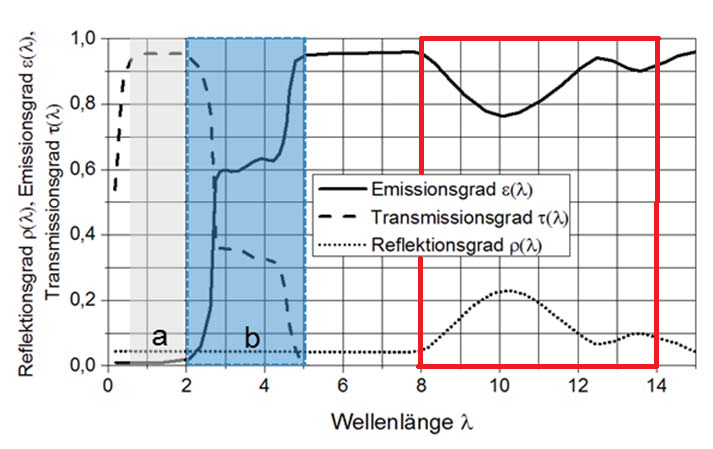
\includegraphics[width=0.6\textwidth]
	{fig/Glas_bearbeitet.png}
	\caption[Emissionsgrad in Abhängigkeit zur Wellenlänge von Glas]{Emissionsgrad in Abhängigkeit zur Wellenlänge von Glas}[\cite{Glas}] 
	\label{fig:Glas}	
\end{figure}

Aus der Grafik geht hervor, dass im Arbeitsbereich des Sensors\footnote[11]{Zwischen 8-14 $\mu$m, in Abbildung \textcolor{red}{rot} markiert} die Transmission ausgeschlossen werden kann. Es besteht jedoch die Schwierigkeit den Emissions- und Reflektionsanteil zu bestimmen, da dieser je nach Wellenlänge schwankt.

Die vorher genannten Einflüsse fallen hauptsächlich ins Gewicht, wenn externe Störquellen wie beispielsweise das Sonnenlicht in einen Aufzug wirken. Ansonsten kann der Aufzug als geschlossenes System betrachtet werden. Lediglich die Aufzugsbeleuchtung wirkt als innere Störquelle.

\begin{figure}[!ht]
	\centering
	\begin{minipage}[b]{0.49\linewidth}
	\centering
	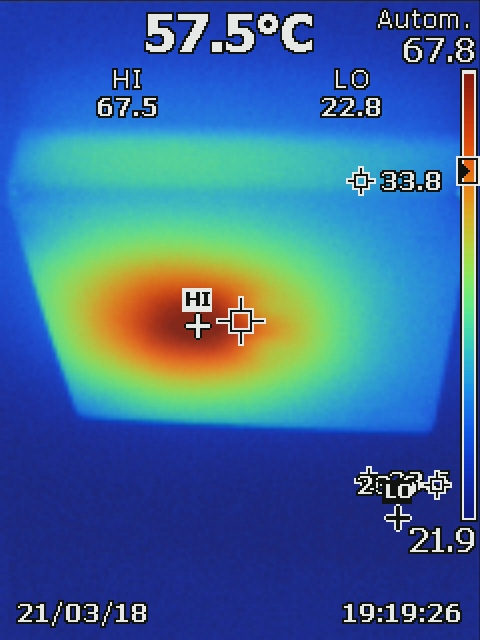
\includegraphics[width=0.5\linewidth]{fig/Lichtquellen.jpg}
	\caption{Wärmebild einer\\ Glühlampen-Beleuchtung}
	\label{fig:lichtquellen}
	\end{minipage}
	\hfill
	\begin{minipage}[b]{0.49\linewidth}
	\centering
	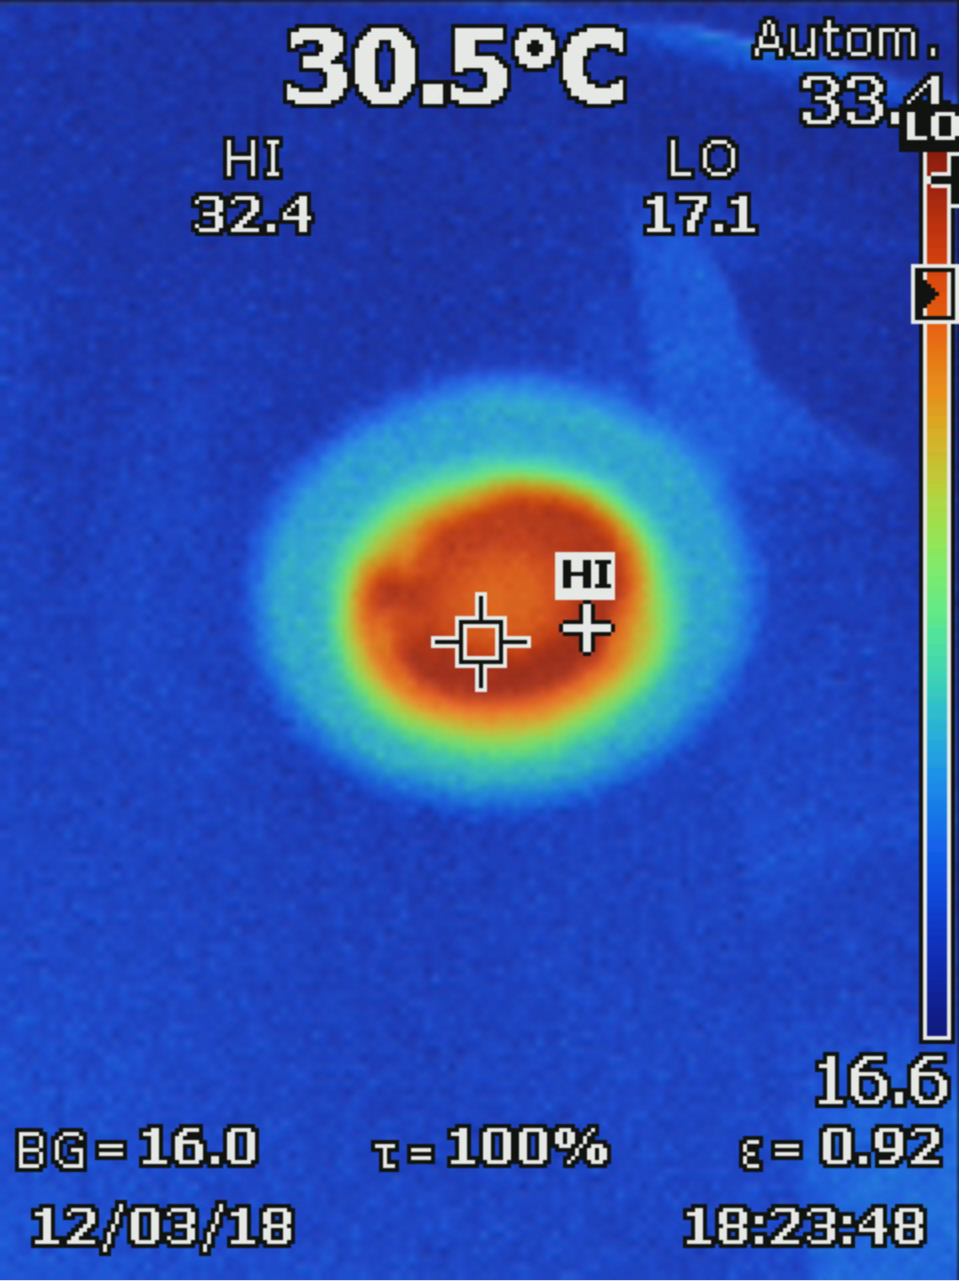
\includegraphics[width=0.5\linewidth]{fig/Lichtquelle.png}
	\caption{Wärmebild einer\\ LED-Spotbeleuchtung}
	\label{fig:m2lichtquelle}
	\end{minipage}
\end{figure}

Da sich die Wellenlängen von üblichen Lichtquellen im tieferen Bereich\footnote[12]{Maximal naher Infrarotbereich [< 3 $\mu$m]} befinden, können die Strahlungen ausgeschlossen werden. Einzig die Betriebstemperatur der Lichtquelle kann den Sensor beeinflussen. Daher empfiehlt sich, den Sensor nicht zu nahe an der Beleuchtung zu positionieren. In Abbildung \ref{fig:lichtquellen}  und \ref{fig:m2lichtquelle} sind unterschiedliche Aufzugsbeleuchtungen mit der Wärmebildkamera TI-125 aufgenommen.



\section{Fazit}

Die Personenerkennung in Aufzügen mit \ac{PIR} Sensoren ist am meisten von der Individualität einer Person abhängig. Faktoren wie Körpertemperatur, Körpergröße und Bekleidung verursachen enorme Differenzen. Dadurch kann kein einheitliches Profil erstellt werden. Da Personenaufzüge Normgrössen besitzen, ist mit dem AMG8834 durch den \ac{FOV} nur einen begrenzten Bereich messbar. Entsprechende Linsenanpassungen können die Problematik lösen. Weitere physikalische Gegebenheiten wie die Umgebungstemperatur oder indirekte Sonneneinstrahlung bewirken veränderte Bedingungen für den Messbereich, welche bei einer Messeinheit berücksichtigt werden müssen. Bei Aufzügen mit Edelstahlverkleidungen können durch den tieferen Emissionsgrad mehr Reflexionen durch externe Störquellen verursacht werden. Die verwendeten Leuchtmittel haben hingegen kaum Einfluss, sofern der Sensor nicht in der Nähe der Lichtquelle platziert wird.     

